\documentclass[oneside,14pt]{extarticle}
\usepackage{cmap}
\usepackage[utf8]{inputenc}
\usepackage[english,ukrainian]{babel}
\usepackage{graphicx}
\usepackage{geometry}
\usepackage{listings}
\usepackage{float}
\usepackage{amsmath}
\usepackage{subfig}
\usepackage{enumitem}
\geometry{
	a4paper,
	left=20mm,
	right=20mm,
	top=15mm,
	bottom=15mm,
}
\lstset{
	language=c,
	tabsize=4,
	keepspaces,
	showstringspaces=false,
	frame=single,
	language=python,
	breaklines=true,
	postbreak=\mbox{{$\hookrightarrow$}\space},
}
\graphicspath{ {./pictures} }
\setlength{\parindent}{4em}

\newcommand\subject{Основи програмування вбудованих систем}
\newcommand\lecturer{професор кафедри ПЗ\\Гавриш В.І.}
\newcommand\teacher{доцент кафедри ПЗ\\Крук О.Г.}
\newcommand\mygroup{ПЗ-32}
\newcommand\lab{1}
\newcommand\theme{Моделювання аналогових $2\pi$- періодичних сигналів рядом Фур’є}
\newcommand\purpose{Наблизити рядом Фур’є аналоговий $2\pi$- періодичний
	сигнал, виконати геометричне зображення функції, якою описано цей сигнал, та
	кривої, яку подано рядом Фур’є. Визначити середню абсолютну похибку
	наближення}

\begin{document}
\begin{normalsize}
	\begin{titlepage}
		\thispagestyle{empty}
		\begin{center}
			\textbf{МІНІСТЕРСТВО ОСВІТИ І НАУКИ УКРАЇНИ\\
				НАЦІОНАЛЬНИЙ УНІВЕРСИТЕТ "ЛЬВІВСЬКА ПОЛІТЕХНІКА"}
		\end{center}
		\begin{flushright}
			\textbf{ІКНІ}\\
			Кафедра \textbf{ПЗ}
		\end{flushright}
		\vspace{120pt}
		\begin{center}
			\textbf{ЗВІТ}\\
			\vspace{10pt}
			до лабораторної роботи № \lab\\
			\textbf{на тему}: <<\textit{\theme}>>\\
			\textbf{з дисципліни}: <<\subject>>
		\end{center}
		\vspace{40pt}
		\begin{flushright}
			
			\textbf{Лектор}:\\
			\lecturer\\
			\vspace{28pt}
			\textbf{Виконав}:\\
			
			студент групи \mygroup\\
			Коваленко Д.М.\\
			\vspace{28pt}
			\textbf{Прийняв}:\\
			
			\teacher\\
			
			\vspace{28pt}
			«\rule{1cm}{0.15mm}» \rule{1.5cm}{0.15mm} 2024 р.\\
			$\sum$ = \rule{1cm}{0.15mm}……………\\
			
		\end{flushright}
		\vspace{\fill}
		\begin{center}
			\textbf{Львів — 2024}
		\end{center}
	\end{titlepage}
		
	\begin{description}
		\item[Тема.] \theme.
		\item[Мета.] \purpose.
	\end{description}

	\section*{Індивідуальне завдання}
	Реалізувати довільною мовою програмування:
	\begin{enumerate}[label=\arabic*)]
		\item підпрограму (процедуру чи функцію), яка дає змогу визначати значення
		потужності сигналу за аналітичним виразом функції та за
		співвідношенням, отриманим у результатом розкладу її в ряд Фур’є;
		\item підпрограми (процедури чи функції), які дають змогу визначити значення
		коефіцієнтів ряду Фур’є;
		\item підпрограму (процедуру чи функцію), яка дає змогу наблизити $2\pi$-
		періодичний сигнал рядом Фур’є з певною точністю, яка пов’язана з
		кількістю доданків N ряду;
		\item підпрограму (процедуру чи функцію) для обчислення середньої
		абсолютної похибки отриманого наближення;
		\item підпрограму (процедуру чи функцію) для зберігання у файлі:
		\begin{enumerate}[label=\alph*)]
			\item параметра N;
			\item визначених коефіцієнтів тригонометричного ряду Фур’є;
			\item середню абсолютну похибку наближення;
		\end{enumerate}
		\item основну програму для виконання наближення заданого $2\pi$ - періодичного
		сигналу тригонометричним рядом Фур'є, яка дає змогу виконати
		геометричне відображення аналогового $2\pi$- періодичного сигналу та його
		наближення кривою, описаною рядом Фур'є.
	\end{enumerate}
	
	\subsection*{Варіант №6}
	
	\begin{equation}
		f(t) = 
		\begin{cases}
			t, & \hspace{-12pt} -\pi < t \leq 0,\\
			2t, & 0 < t < \pi
		\end{cases}\nonumber
	\end{equation}

	\section*{Теоретичні відомості}
	
	Апроксимація – це створення функції, яка буде спрощувати вхідну складну функцію. Тобто якщо задана функція є доволі складною, до неї можна застосувати апроксимацію, яка знайде простішу функцію, яка буде максимально подібна до вхідної.
	
	Апроксимація передбачає створення поліномів такого типу:
	
	\begin{equation}
		f(x)=c_0+c_1x+...+c_nx^n\nonumber
	\end{equation}
	
	Так як сигнали завжди періодичні, отже і спрощувати їх потрібно періодичною функцією, яка є поліномом, ця функція між періодами може мати розриви. Для усунення цих розривів застосовують ряди Фур’є.
	
	Сам по собі ряд Фур’є – це представлення складної функції сумою простіших. Таке визначення є дуже загальним, але так як для апроксимації сигналів використовуються тригонометричні функції (так як вони є періодичними), то і ряд Фур’є має бути тригонометричним.
	
	Такий ряд має вигляд:
	
	\begin{gather}
		f_a(x)=\frac{a_0}{2}+\sum_{k=1}^{\infty}(k\cos(kx)+b_k\sin(kx))\nonumber
	\end{gather}
	
	Де $a_0$, $a_k$, $b_k$ визначають так:
	
	\begin{gather}
		a_k=\frac{1}{\pi}\int_{-\pi}^{\pi}f(x)\cos(kx)dx\nonumber\\
		b_k=\frac{1}{\pi}\int_{-\pi}^{\pi}f(x)\sin(kx)dx\nonumber
	\end{gather}
	
	\section*{Хід роботи}	

	\subsection*{Код програми}
	Файл \textit{main.py}:
	{\small
		\begin{lstlisting}
import numpy as np
import matplotlib.pyplot as plt
import math
import json

# Define the original signal function
def f(t):
	if -np.pi < t <= 0:
		return t
	elif 0 < t < np.pi:
		return 2 * t
	else:
		return 0

# Function to compute Fourier coefficients
def fourier_coefficients(f, N):
	a0 = (1/np.pi) * np.trapz([f(t) for t in np.linspace(-np.pi, np.pi, 1000)], np.linspace(-np.pi, np.pi, 1000))
	an = lambda n: (1/np.pi) * np.trapz([f(t) * np.cos(n*t) for t in np.linspace(-np.pi, np.pi, 1000)], np.linspace(-np.pi, np.pi, 1000))
	bn = lambda n: (1/np.pi) * np.trapz([f(t) * np.sin(n*t) for t in np.linspace(-np.pi, np.pi, 1000)], np.linspace(-np.pi, np.pi, 1000))
	coefficients = {'a0': a0, 'an': [an(n) for n in range(1, N+1)], 'bn': [bn(n) for n in range(1, N+1)]}
	return coefficients

# Function to approximate the signal using Fourier series
def fourier_series_approximation(t, coefficients, N):
	a0 = coefficients['a0']
	an = coefficients['an']
	bn = coefficients['bn']
	approximation = a0/2 + sum([an[n-1]*np.cos(n*t) + bn[n-1]*np.sin(n*t) for n in range(1, N+1)])
	return approximation

# Function to compute the mean absolute error of the approximation
def mean_absolute_error(original, approximation):
	return np.mean(np.abs(np.array(original) - np.array(approximation)))

# Function to save results to a file
def save_results(N, coefficients, error):
	with open("fourier_results.json", "w") as file:
	results = {'N': N, 'coefficients': coefficients, 'error': error}
	json.dump(results, file, indent=2)

# Main program
def main():
	N = 6  # Number of terms in the Fourier series
	t_values = np.linspace(-np.pi, np.pi, 1000)
	original_signal = [f(t) for t in t_values]
	coefficients = fourier_coefficients(f, N)
	approximation = [fourier_series_approximation(t, coefficients, N) for t in t_values]
	error = mean_absolute_error(original_signal, approximation)
	save_results(N, coefficients, error)

	plt.figure(figsize=(10, 6))
	plt.plot(t_values, original_signal, label='Original Signal')
	plt.plot(t_values, approximation, label='Fourier Approximation', linestyle='--')
	plt.title(f'Fourier Series Approximation with N={N}')
	plt.legend()
	plt.show()

if __name__ == "__main__":
	main()\end{lstlisting}
	}
	
	\subsection*{Виконання програми}
	
	\begin{figure}[H]
		\centering
		\vspace{-30pt}
		\includegraphics[scale=0.58]{1}
		\vspace{-30pt}
		\caption{Геометричне зображення сигналу та його наближення кривою, описаною рядом Фур’є для $N=100$ на інтервалі $x\in(-4\pi;4\pi]$.}
	\end{figure}
	
	\begin{figure}[H]
		\centering
		\vspace{-30pt}
		\includegraphics[scale=0.58]{2}
		\vspace{-30pt}
		\caption{Геометричне зображення сигналу та його наближення кривою, описаною рядом Фур’є для $N=100$ в точці розриву $(x=-\pi)$.}
	\end{figure}
	
	\begin{figure}[H]
		\centering
		\vspace{-30pt}
		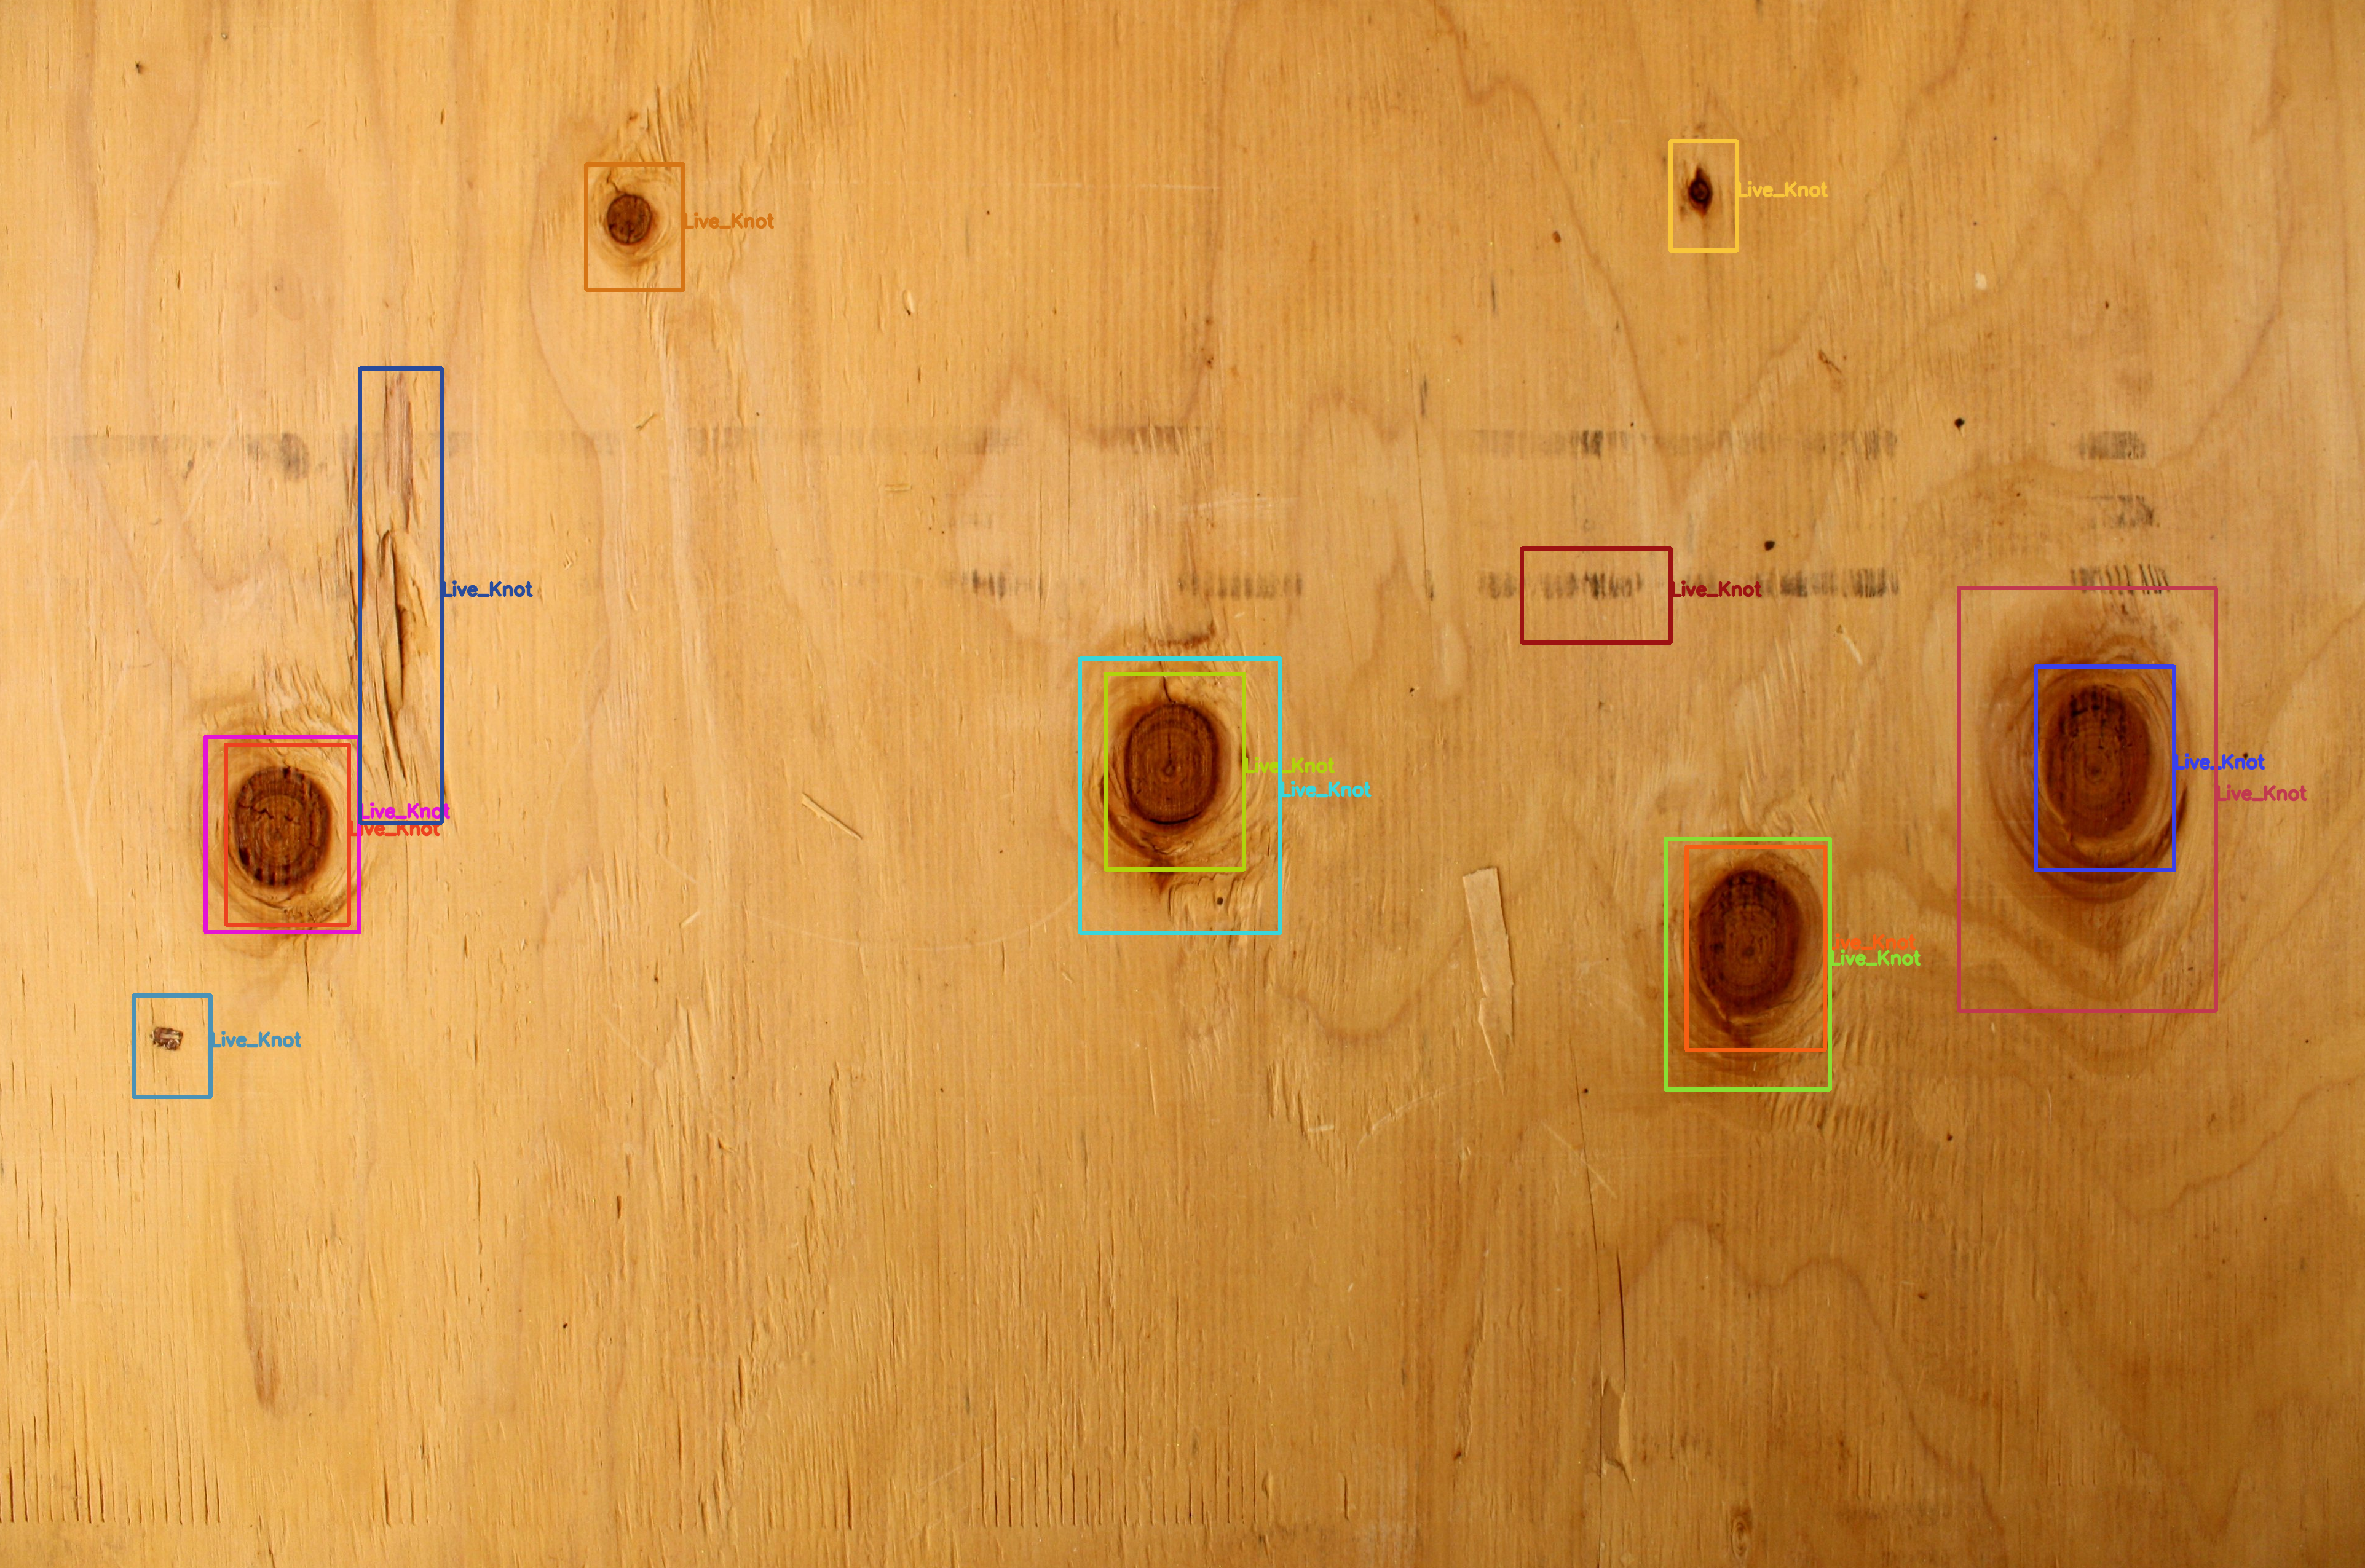
\includegraphics[scale=0.58]{3}
		\vspace{-30pt}
		\caption{Геометричне зображення сигналу та його наближення кривою, описаною рядом Фур’є для $N=100$ в точці розриву $(x=-\pi)$.}
	\end{figure}
	
	\begin{figure}[H]
		\centering
		\vspace{-30pt}
		\includegraphics[scale=0.58]{4}
		\vspace{-30pt}
		\caption{Геометричне зображення сигналу та його наближення кривою, описаною рядом Фур’є для $N=100$ в точці $(x=0)$.}
	\end{figure}
	
	\begin{figure}[H]
		\centering
		\vspace{-30pt}
		\includegraphics[scale=0.58]{5}
		\vspace{-20pt}
		\caption{Вивід у файл після виконання програми для $N=10$.}
	\end{figure}
	
	\begin{table}[H]
		\centering
		\renewcommand{\arraystretch}{1.5}
		\begin{tabular}{|c@{\hspace{15pt}}|c@{\hspace{15pt}}|}
			\hline
			$N$ & Похибка \\ \hline
			10 & 0.2929 \\ \hline
			50 & 0.0795 \\ \hline
			100 & 0.0434 \\ \hline
		\end{tabular}
		\caption{Порівняння середньої абсолютної похибки наближення для різних значень $N$.}
	\end{table}
	
	\section*{Висновки}
	Під час виконання лабораторної роботи я розробив обчислювальний алгоритм,
	реалізований алгоритмічною мовою Python, що дає змогу наблизити аналоговий $2\pi$ періодичний сигнал рядом Фур’є та визначити середню абсолютну похибку наближення. У результаті досліджень досягнуто значення середньої абсолютної похибки $0.0434$ для $100$ доданків ряду Фур'є.
	    
\end{normalsize}
\end{document}
